\chapter{LDoS攻击原理与形式介绍}
\label{cha:LDoS}

本章的主要内容是对LDoS攻击进行探讨。首先对LDoS攻击原理进行说明。接下来,对LDoS攻击模型进行分析与说明。最后,对LDoS攻击的各类攻击形式进行分析和探讨。

\section{LDoS攻击原理}
\label{chap3:LDoSstate}

\subsection{TCP拥塞控制机制和超时重传机制}

此部分的主要内容为分析传输控制协议(Transmission Control Protocol,TCP)的拥塞控制机制与超时重传机制。首先讨论了不同时期提出的TCP拥塞控制机制,然后对超时重传机制(Retransmission Time Out, RTO)进行分析,探讨超时重传机制对TCP流的影响。

TCP协议是保证数据可靠的协议。对于任何基于TCP协议的数据流,都需要TCP拥塞控制机制,因为该机制可以对网络进行有效的调节。在网络中,所有的流都想让自己的数据尽快的传输,但是,所有流尽可能传输的结果容易造成路由器或者链路的负载过大,引发网络拥塞,导致所有流都无法传输数据。因此,网络拥塞控制对于网络是必不可少的,而TCP拥塞控制是为了给TCP流提供合适的竞争方式。

在传输层中TCP协议实现了拥塞控制机制。TCP拥塞控制机制也并非一成不变的,针对不同的场景,TCP拥塞控制的策略也会不同,很多研究对TCP拥塞控制机制进行了探索。

最早的拥塞控制机制是1988年由Jacobson.V\cite{Jacobson1988Congestion}提出的TCP Reno版本,该方案的主要是由慢启动、拥塞避免、快重传和快恢复四个部分组成,大部分的拥塞控制方案都是以该方案作为基础进行提升的,由于该方案设计的时候有些方面未曾考虑,因此,该方案仅适用于低延迟、低带宽的网络。
在1994年由O’Malley.S.W\cite{O1994TCP}提出的TCP Vegas版本,该方案通过RTT来精准的预测带宽的变化,判断网络的可用带宽。不过,该方案适用于只存在这一种算法的时候。
在2008年,由Ha.S\cite{Ha2008CUBIC}提出的TCP Cubic方案,该方案使用立方函数作为拥塞窗口的增长函数,因此能够在不出现丢包的情况下,保持自己的传输速率。该方案能够尽可能的利用网络剩余带宽,适用于高带宽、丢包少的网络。
2017年由Cardwell.N\cite{Cardwell2017BBR}提出的TCP BBR版本,该算法在谷歌使用之后,极大的提升了数据传输性能。该算法认为当网络中的数据包总量高于网络中可存放数据包总量的时候会产生拥塞,就会限制窗口,因此,在带宽高、延迟高还有一定丢包率的情况下,降低时延并且保证带宽。
此外,2013年由Winstein.K\cite{Winstein2013Remy}提出的Remy算法采用机器学习的方式生成拥塞控制形式。因此,该算法适用于复杂的网络环境。

拥塞控制机制并非一成不变的,不同的方案有不同的适应场景,但是,这些方案都遵循着超时重传机制。在网络极其拥塞的情况下,TCP协议的发送端与接收端都收不到数据包,此时为了保证数据稳定的传输,TCP协议的发送端会进入指数退避阶段,将发送窗口改为1,避免网络进一步拥塞。在超时重传机制中,TCP流依靠RTO计时器来不定期探测网络拥塞状况。在TCP协议运行的过程中,RTO计时器中的值是由根据往返时间(Round-Trip Time,RTT)实时计算得到的。

TCP的发送端维持两个变量,平滑往返时间(Smoothed Round-Trip Time, SRTT)和往返时间变化量(Round-Trip Time VARiation, RTTVAR)。根据RFC2988\cite{2000Computing}的设定,RTO的实时计算结果与SRTT、RTTVAR两个变量相关。当TCP的发送端与接收端完成一次测量RTT之后,发送端将RTO计时器设置为3秒。
当第一次测量获得的RTT,记为$R'$,主机设置SRTT = $R'$,RTTVAR = $R' / 2$,RTO = SRTT + max(G, 4RTTVAR),此处的G被标记为时钟粒度(一般情况下,$\leq$100毫秒)。当获得一个RTT的值$R'$之后,RTTVAR和SRTT的计算公式如下:
%记为

\begin{center}
    RTTVAR = (1 - $\beta '$) RTTVAR + $\beta '$ |SRTT - $R'$|
\vspace{-0.1in}
\end{center}

\begin{center}
    SRTT = (1 - $\alpha '$) SRTT + $\alpha ' R'$
\end{center}

其中,有文献\cite{Jacobson1988Congestion}推荐设置$\alpha '$ = 1/8, $\beta '$ = 1/4。


通过对RTTVAR和SRTT进行更新之后,TCP发送端RTO的计算公式如下:
\begin{center}
    RTO = max(minRTO, SRTT + max(G,4 RTTVAR))
\end{center}

在Linux系统中,一般而言RTO计时器的最小值(minRTO)设置为0.2秒,因此,在推荐的参数中,延迟低的网络RTO基本是0.2秒。

接下来,对超时重传管理机制中RTO计时器进行控制的流程进行分析。若是在某一时刻$t_0$,一个序号为$n$的数据包有TCP的发送端发送,此时一个初始RTO值设为0.2秒的RTO计时器开始计时,如果$n$号的数据包丢失了或者说接收端重复发送的三个ACK包都没被发送包接收。当RTO计时器算到0.2秒的时候,则这个流就会被认为超时。此时,发送端进入指数退避阶段,发送端将拥塞控制的窗口置为1,并且让RTO计时器的值加倍,变为400毫秒,重传序号为$n$的未曾接收到ACK的数据包,并且重置RTO计时器为新的RTO的值。
%对超时重传管理机制通过(中)RTO计时器进行控制的流程进行分析
若是序号为$n$的数据包再次丢失,则发送端持续保持,发送端将保持在指数退避阶段,而RTO计时器将会等待400毫秒。也就是说在$t_0$ + 0.6s的时候,RTO的值将被设为800毫秒,并重复此过程。

若是序号为$n$的数据包的数据包成功的$t_0$ + 0.2s之前接收到该数据包,例如在$t$+ RTT的时刻接收到$n$号数据包,则TCP发送端退出指数退避阶段并将RTO的值置为0.2秒,又开始正常的传输。

\subsection{LDoS攻击原理}
此部分的主要内容对LDoS攻击原理进行分析,阐述如何利用TCP的超时重传机制对来实现DoS攻击。

上述的超时机制对于拥塞控制是十分重要的,因为在网络十分拥塞的情况下,发送少量的数据包先进行探测网络的可达性是必要的。但是,这样的超时重传机制也会给网络带来很大的风险,比如给特定的低速率攻击能够利用该机制对TCP流产生极大的影响。

若是一个攻击者针对TCP流,通过发送周期性的短时间高速突发来迫使该流重复进入超时重传状态。攻击的突发持续时间必须得超过RTT的时间,需要RTO为攻击的周期的整数倍数,例如,RTO,RTO/2,RTO/3等。受害者的吞吐量被限制待到近乎为0的程度。与此同时,由于该攻击的平均速率较低,不容易被DoS的对抗机制所检测。

\begin{figure}
    \centering
    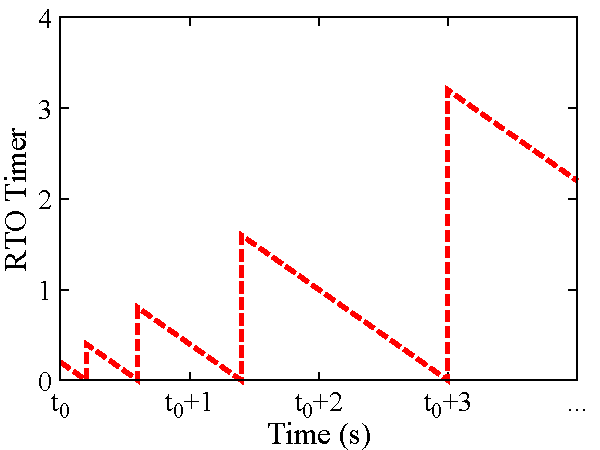
\includegraphics[scale=0.75]{RTO_timer}
    \caption{$t_0$时刻发动LDoS攻击之后,RTO计时器变化情况}
    \label{fig:rto-timer}
\end{figure}

首先考虑最简单的情况,若是一个攻击者仅仅针对一条TCP流进行攻击,攻击者在$t_0$时刻开始展开攻击,开始发送短时间的高速突发,就像图\ref{fig:rto-timer}展示的那样,根据RTO计时器的初始值为0.2秒,该TCP流会等待0.2秒。如果攻击者在$t_0$ + 0.2和$t_0$ + 0.2 + 2RTT的时间内进行短时间的突发流进行攻击,则TCP流将不得不等待额外的0.4秒。通过在$t$= $t_0$ + 0.6, $t_0$ + 1.4等点创造类似的攻击,就能够不断迫使该TCP流进入超时重传状态。因此,可以得到针对某一特定TCP流的DoS攻击流的形式,如图\ref{fig:rate-min-LDoS}所示。

\begin{figure}
    \centering
    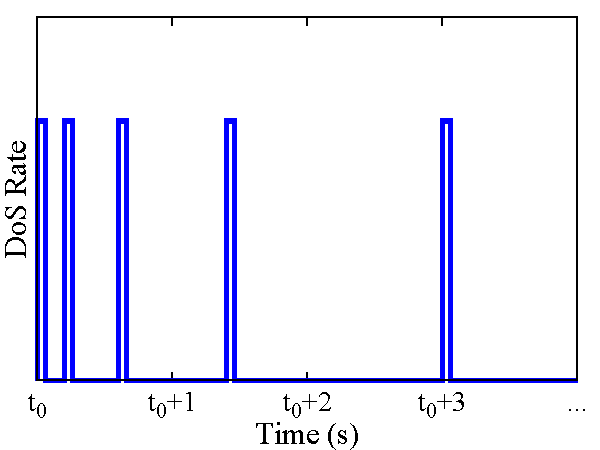
\includegraphics[scale=0.75]{rate-min-LDoS}
    \caption{高效的低速攻击方案}
    \label{fig:rate-min-LDoS}
\end{figure}

图\ref{fig:rate-min-LDoS}的攻击形式能够以最小的平均攻击速率使一个TCP流不断进入超时重传状态。但是,该形式却存在一个很大的弊端,若是在某一次攻击突发没有让ACK包被丢弃,则RTO计时器会重置为初始值,这样会使得该形式失效。因此,该形式虽然效率高,平均速率低,但是,并不适合于用作LDoS的基础形式。


\section{LDoS攻击模型}
\label{chap3:LDoS-model}
LDoS攻击形式需要一定的稳定性,不能因为偶尔出现的特殊情况就失去效果,考虑到这一点,使用周期性“方波”形式的UDP流作为LDoS攻击的基础形式能够获得比较好的效果。如图\ref{fig:LDoS}所示,其中攻击者可以通过发送周期为$T$,每次突发持续时间为$L$,突发速率为$R$的LDoS攻击流来对TCP流进行攻击。此时,可以用三个参数($T$,$L$,$R$)来描述LDoS攻击流。使用$\eta$来表示$\frac{L}{T}$的比值。

在这里,先以超时重传机制作为目标,分析LDoS攻击模型。LDoS攻击迫使TCP流进入超时重传状态是需要满足一定的条件的。首先,速率$R$必须足够大来引起丢包,也就是说,$R$与其他的流量混合起来一定要超过链路容量。其次,突发持续时间$L$必须足够长来引起丢包,但是也要足够短来避免检测。RTO计时器的初始值必须是周期$T$整数倍,为了使攻击的平均流量最小,本文将$T$设为minRTO,这样就能够满足LDoS攻击实现的条件。

\begin{figure}
    \centering
    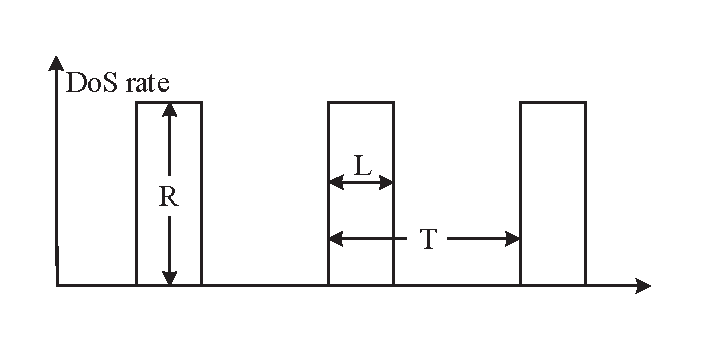
\includegraphics[scale=0.75]{LDoS}
    \caption{LDoS攻击形式}
    \label{fig:LDoS}
\end{figure}

前面讨论了针对一条攻击流的考虑LDoS攻击的情景,可以得到LDoS攻击模型,如图\ref{fig:model}所示,n条拥有不同RTT的TCP流和一条LDoS攻击流通过一个瓶颈队列。将RTT$_{i}$标记为第i条TCP流的RTT,其中i=1,…,$n$。LDoS攻击起效需要满足下面的条件:
\begin{itemize}
    \item 突发持续时间$L \geq RTT_i $
    \item minRTO > SRTT$_i$ + 4*RTTVAR$_i$
\end{itemize}

通过之前的分析可以得出一个结论,周期性的高速突发能够创造一段“停滞”状态,在这种状态下,丢包率很高,如果这种状态维持的时间超过RTT的时间规模,即$L \geq RTT_i$,则由LDoS的攻击突发引起的拥塞将维持足够长的时间来迫使所有的TCP流进入超时重传状态。除此之外,当且仅当minRTO > SRTT$_i$ + 4*RTTVAR$_i$的时候,则所有TCP流的RTO计时器的值就会统一为minRTO,这样攻击者就能够知道TCP流的RTO计时器的值。在这种情况下,能够排除影响LDoS攻击的两个重要的问题,第一个问题是不同的TCP流RTT不同;第二个问题是不同的TCP流RTO计时器的值不同。这样,LDoS攻击就能够对满足这两个条件的TCP流进行攻击。LDoS攻击不能迫使满足不了条件的TCP流吞吐量降为0,但是也能够占用部分TCP流的带宽,降低TCP流的吞吐量。综上所述,LDoS攻击能够对满足条件的TCP流有非常好的攻击效果,对不满足条件的TCP流效果有所下降。在生成LDoS攻击流量的时候需要注意设置相应参数尽可能覆盖更多的TCP流。



% 接下来,考虑如果有TCP流不满足上述两个条件其中任何一个甚至两个都不满足,LDoS攻击的效果就会不一样。如果一些TCP流只有一部分满足上面两个条件,则他们的吞吐量将会降低至近乎为0的程度,而不满足上述条件的则吞吐量下降,下降的之后的标准化吞吐量由公式\ref{equ:thputsurvive}来描述。

% \begin{equation}
%     \label{equ:thputsurvive}
%     NT = \frac{\lceil \frac{minRTO}{T}\rceil T - minRTO}{T}.
% \end{equation}

\begin{figure}
    \centering
    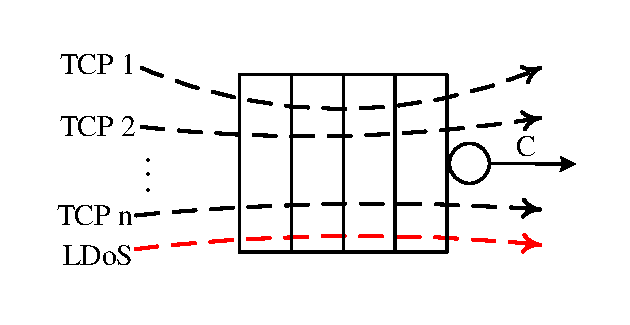
\includegraphics[scale=1]{queue}
    \caption{LDoS攻击模型}
    \label{fig:model}
\end{figure}

\section{各种类型的LDoS攻击}
\label{chap3:LDoStypes}
在LDoS攻击的基础形式被提出来之后,各种类型的LDoS攻击被提出来,根据目标的不同设定相应的参数能达到不同的攻击效果,例如基于超时重传机制的LDoS就能够迫使TCP流不断地进入超时重传机制,基于TCP的和式增加,积式减少(Additive Increase Multiplicative Decrease,AIMD)机制的LDoS能够迫使TCP流频繁地进入快恢复的状态。

根据Luo.X\cite{Luo2005OnAN}提出的方案,有两种LDoS攻击类型:第一种LDoS攻击可以继续利用超时重传机制降低TCP流的吞吐量;第二种LDoS攻击利用TCP的AIMD机制来降低TCP流的吞吐流量。第一种LDoS攻击同样需要图\ref{fig:LDoS}作为基础模型,$R$需要达到足够引起丢包,$L$需要长到引发ACK包丢失,$T$设定为比minRTO的值大一些。这样的LDoS攻击能够让TCP大部分的时间处于超时重传状态中,TCP流吞吐量依然降低了,但是并不能到近乎为0的程度。该方案的RTO计时器变化曲线如图\ref{fig:rto-timer-1}所示。由于该方案不需要与minRTO成倍数关系,所以比较好实现。第二种LDoS攻击是利用AIMD机制完成攻击。在通常的AIMD算法中,如果某一TCP流的滑动窗口大小为W,则由于一次短时间的高速突发引起该TCP流的数据包丢失,但是相应的ACK数据包到达了发送端,则TCP流不会进入超时重传状态,而TCP流的滑动窗口会下降至W/2。从此之后,该TCP流的滑动窗口大小每个RTT都增长1。针对TCP的AIMD机制的LDoS攻击同样被用来降低TCP流的吞吐量。攻击形式依然如图\ref{fig:LDoS}所示,相同的是$R$依然需要达到足够引起丢包,不同的是,$L$需要长到引发部分丢包即可,$T$可以设定为比较小的值这样,TCP流就会不断地减小滑动窗口大小。上述两种方式都能有效的降低TCP流的吞吐量。

\begin{figure}
    \centering
    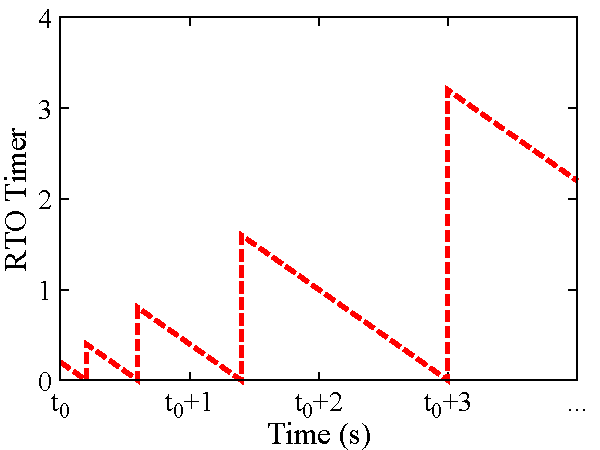
\includegraphics[scale=0.75]{RTO_timer}
    \caption{被新型利用超时重传机制的LDoS攻击的TCP流RTO计时器变化}
    \label{fig:rto-timer-1}
\end{figure}

也有研究\cite{b2}提出针对于BGP协议的LDoS攻击。由于BGP边界路由器之间使用TCP连接来交换可达性信息。在这样的情况下,使用对TCP流有很好效果的LDoS攻击将会对BGP会话的运行造成很大的影响。LDoS攻击对BGP会话的直接影响有两个:吞吐量下降和会话重置。第一个影响是吞吐量下降,因此BGP传递的信息会减少很多,BGP的更新速率将会非常缓慢,所以LDoS攻击大大降低了BGP的收敛速率。第二个影响就更加严重,BGP会话会重启,若是LDoS攻击流量持续时间足够长就能够引发BGP会话计时器超时,重启会话。BGP会话重启也将会加大的影响BGP的控制平面。

有文献\cite{Maci2007Evaluation}提出针对服务器队列的LDoS攻击。针对服务器的LDoS攻击首先对服务器进行洪泛攻击,让恶意请求使服务器的队列一处,然后,使用LDoS攻击形式去对服务器进行攻击,周期性的发送恶意请求给服务器,在每次预测到服务器的队列没有完全被使用的时候,就在那段时间里不断发送请求给服务器,直到服务器队列再次溢出。攻击的周期为一个服务器接受请求到下发回复的时间长度。该类LDoS攻击通过消耗服务器的队列资源使服务器拒绝服务,而且由于发送请求的速率相对比较低且均为合法流量,因此,难以被检测。

还存在有针对应用层HTTP协议的的LDoS攻击\footnote{https://blogs.akamai.com/2013/09/slow-dos-on-the-rise.html}。该类攻击有三种类型:Slow HTTP Headers,Slow HTTP Post和Slow Read Attack。这三种类型攻击都是通过发送大量合法的请求给服务器来创造大量的服务器连接,并发送周期性的合法请求来长期维持这些连接,在大量占用了服务器链接资源池的资源之后,一直不释放,则链接资源池被沾满,造成服务器的服务拒绝攻击。而且由于合法请求造成的资源被占用,难以被释放。
%占用-释放
\section{低速率分布式服务拒绝攻击}


前文所分析的LDoS攻击都是有某一主机作为攻击者集中实现的,这样便于部署攻击并保证攻击形式能够按照要求实现。低速率分布式服务拒绝(Low-rate Distributed Denial of Service, LDDoS)攻击作为LDoS的分布式部署方式,相较于单攻击源的LDoS攻击拥有很多的优势。首先,若是想对性能比较好的交换机上使用LDoS攻击,单主机的性能可能达不到要求,需要多主机联合攻击。其次,作为分布式LDoS的每个攻击主机拥有更加低的平均速率,更加不易被检测出来。

部署分布式LDoS攻击是需要前提条件的,只有满足了一定条件才能实现分布式攻击。假设多个攻击主机想联合对某条TCP流$f$进行攻击,则需要这些攻击主机在该TCP流经过的一个交换机$s_r$上的链路$l$进行攻击,且攻击主机的流量需要以一定的规则汇聚到$l$上。所以,攻击主机需要满足两个条件:(1)每个攻击主机都有一条攻击路径经过$l$;(2)所有主机需要计算好时间,使得流量到$l$处时刚好形成LDoS攻击。除此之外,攻击主机还需要发送足够的突发流量来拥塞这个瓶颈链路$l$,并设置好攻击周期来避免检测。

在满足了上述两个条件之后,同步的分布式LDoS攻击就具备了拥塞TCP流的能力。在多个攻击主机上运行的LDoS攻击与单一攻击源的单独流量更低,也存在很多不同的形式,接下来,以两个主机联合攻击来展示迫使TCP流持续保持超时重传状态的分布式LDoS攻击。


\begin{figure}
    \vspace{-0.2in}
    \begin{subfigure}{1\textwidth}
        \centering
        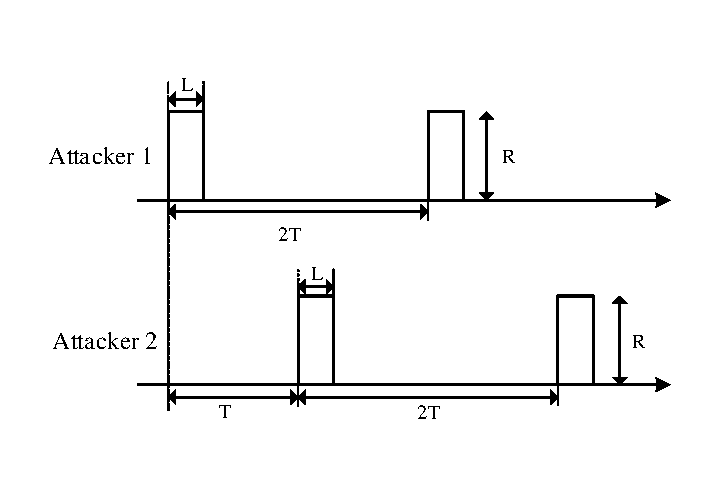
\includegraphics[scale=0.75]{lddos2}
        \caption{方案一}
        \label{fig:lldos1}
    \end{subfigure}

    \begin{subfigure}{1\textwidth}
        \centering
        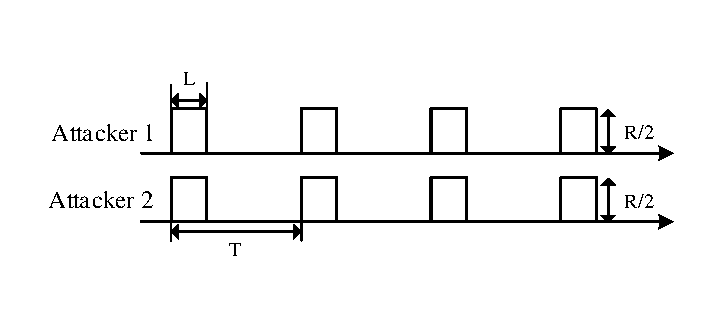
\includegraphics[scale=0.75]{lddos3}
        \caption{方案二}
        \label{fig:lldos2}
    \end{subfigure}

    \begin{subfigure}{1\textwidth}
        \centering
        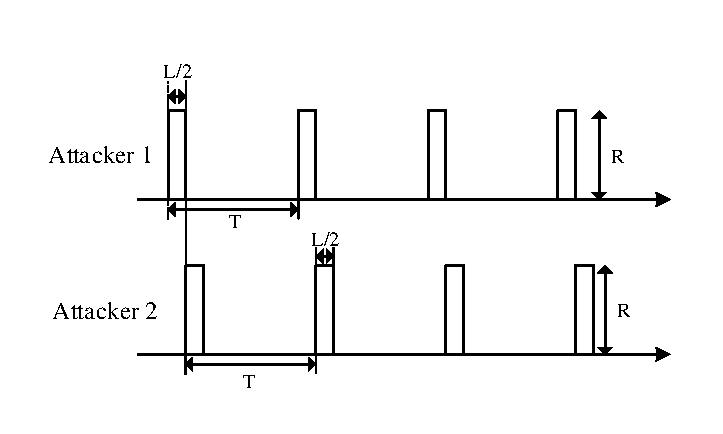
\includegraphics[scale=0.75]{lddos1}
        \caption{方案三}
        \label{fig:lldos3}
    \end{subfigure}


    \caption{分布式LDoS攻击}
    \label{ffig:lldos}
\end{figure}


% \begin{figure}
%     \centering
%     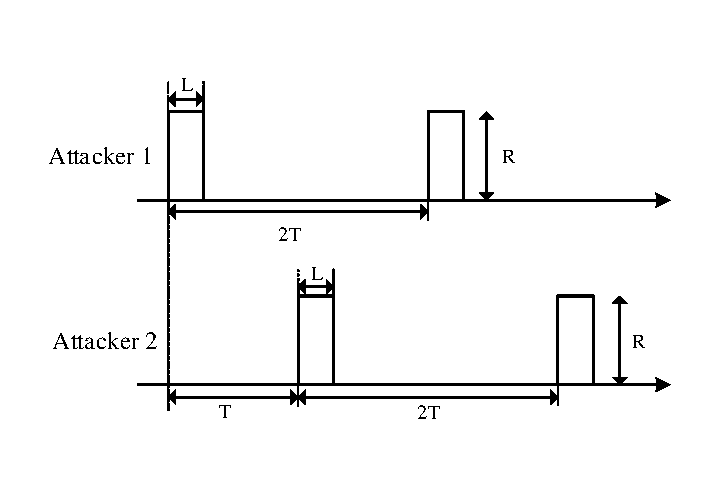
\includegraphics[scale=0.75]{lddos2}
%     \caption{分布式LDoS攻击的第一种方案}
%     \label{fig:lldos1}
% \end{figure}
图\ref{fig:lldos1}为分布式方案一,将该方案的两个流聚合,就可以得到一个参数为($R$,$L$,$T$)的LDoS。首先对第一种方案进行分析,假设攻击者1在零时刻发动了突发速率为$R$,周期为$2T$,每次突发持续时间为$L$的LDoS攻击,则TCP流$f$由于攻击进入超时重传状态。每次$t$ = 2i * T(i=0,1,2…)时刻的$f$可能出现的ACK数据包由于攻击者1的攻击流的拥塞而丢弃。攻击者2需要在$T$时刻发动突发速率为$R$,周期为$2T$,每次突发持续时间为$L$的LDoS攻击,则每次$t$ = (2i + 1) * T(i=0,1,2…)时刻的$f$可能出现的ACK数据包由于攻击者2的攻击流的拥塞而丢弃。至此,由于两个攻击者的拥塞,TCP流$f$的所有可能接受的的ACK报都丢失了,因此,该TCP流持续保持超时重传状态。

% \begin{figure}
%     \centering
%     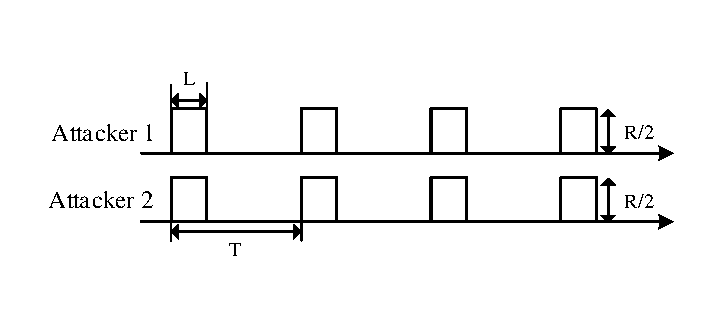
\includegraphics[scale=0.75]{lddos3}
%     \caption{分布式LDoS攻击的第二种方案}
%     \label{fig:lldos2}
% \end{figure}

图\ref{fig:lldos2}为分布式方案二。攻击者1在零时刻发动突发速率为$R/2$,周期为$T$,每次突发持续时间为$L$的LDoS攻击,若是只有攻击者1,则由于攻击突发速率不足,不能使队列拥塞并造成TCP流的丢包,所以,需要攻击者2与攻击者1在零时刻同步发动突发速率为$R/2$,周期为$T$,每次突发持续时间为$L$的LDoS攻击,攻击突发速率足够,因此,交换机的队列拥塞造成TCP流的包完全丢失,最终持续进入超时重传状态。

% \begin{figure}
%     \centering
%     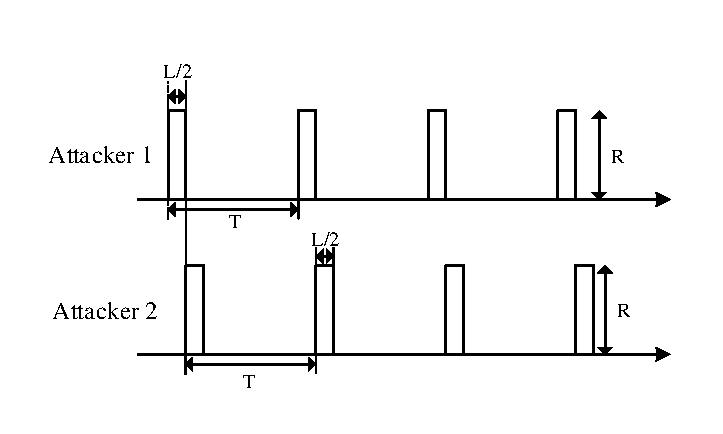
\includegraphics[scale=1=0.75]{lddos1}
%     \caption{分布式LDoS攻击的第三种方案}
%     \label{fig:lldos3}
% \end{figure}

图\ref{fig:lldos3}为分布式方案三。攻击者1在零时刻发动突发速率为$R$,周期为$T$,每次突发持续时间为$L/2$的LDoS攻击。若只有攻击者1的攻击,则由于突发持续时间不足,导致TCP流的ACK包可以为TCP发送端接收到,无法迫使TCP流进入超时重传状态。因此,需要攻击者2在$L/2$时刻,也发动突发速率为$R$,周期为$T$,每次突发持续时间为$L/2$的LDoS攻击。由于攻击者2的攻击在攻击者1结束的时候刚好出现,因此,延续了攻击者1的LDoS攻击的效果,TCP流的ACK包由于攻击者2的拥塞而丢失,所以该TCP流被迫进入超时重传机制。

以上三种方案分别在突发持续时间、突发峰值速率、突发周期上进行了分布式探索,三种方案都能够迫使TCP流保持超时重传状态,而且每个攻击主机都平均攻击速率相较于单一主机都有所下降,这样更易于逃避DoS防御机制的检测。

